\documentclass[conference]{IEEEtran}
\pagestyle{plain}

\usepackage{graphicx}
\usepackage{amsmath,amssymb}
\usepackage{algorithmic}
\usepackage{textcomp}
\usepackage{hyperref}



\begin{document}

\title{AI-Driven Multi-Purpose Autonomous Robotics System for Real-Time Aquaculture Security and Flood Mapping Using Amphibious UGVs and UAVs}

\author{
    Ajharul Abedeen \\
    Software Engineer \\
    Founder, Gobeshona (\url{gobeshona.org}) \\
    \href{mailto:ajharulabedeen@gmail.com}{ajharulabedeen@gmail.com} \\
    \href{mailto:ajharulabedeen@gobeshona.org}{ajharulabedeen@gobeshona.org}
}

\date{\today}

\maketitle

\begin{abstract}
In flood-prone regions, aquaculture systems like Gher farming and broader public infrastructure face serious challenges from climate-induced floods and environmental threats, including water contamination and intentional poisoning. This research proposes a novel, multi-purpose autonomous robotics system integrating Unmanned Aerial Vehicles (UAVs), amphibious Unmanned Ground Vehicles (UGVs), AI, and IoT for comprehensive Gher farming security and flood disaster management. 
\\\\Uniquely designed for dual-functionality, the system transitions seamlessly between peace-time aquaculture monitoring and real-time flood response. In the aquaculture context, the system combines UAV-based aerial reconnaissance, sonar-equipped amphibious UGVs for fish stock monitoring, and IoT sensors to detect water quality anomalies, deploying autonomous barriers or drones to contain and remediate any contamination events. During floods, the same system repurposes to map submerged areas, monitor water quality in flood zones, and provide updated data for emergency response teams. Expected outcomes include improved aquaculture resilience, enhanced disaster preparedness, and an adaptable, globally applicable solution that bridges agricultural security and disaster management. This innovative integration of robotics establishes a model for multi-functional, scalable solutions in vulnerable regions.
\end{abstract}

\section{\textbf{Introduction}}

This research proposal addresses the intertwined challenges of agricultural monitoring and flood management, proposing a multi-purpose autonomous system that integrates these functions to serve various regions affected by both climate change and natural disasters. While Bangladesh is used as an ideal case study due to its frequent flooding and reliance on Gher/Fish farming, the system is designed to be scalable and adaptable to other flood-prone and agriculturally vulnerable regions around the world.

The introduction is structured to first provide an overview of Gher farming, a system commonly used in Bangladesh and similar coastal and freshwater regions, focusing on its significance, structure, and the common challenges it faces, such as water quality issues, theft, poisoning, and environmental threats. Following this, the focus will shift to flood management, discussing the increasing frequency and intensity of floods driven by climate change, which pose significant challenges to urban and rural areas alike, including agricultural systems like Gher farms.

The final part of this introduction will establish a connection between these two domains, highlighting how seasonal flooding impacts agricultural systems and how the same technological system can be adapted for year-round use—monitoring and protecting farms during peace times and providing real-time mapping and monitoring during flood emergencies. This integrated approach underscores the potential for developing a cost-efficient, scalable solution that can benefit both agriculture and disaster management across a variety of geographical contexts, offering a novel perspective on addressing these challenges simultaneously.



\subsection{\textbf{Gher Farming: A Unique and Sustainable Agricultural System in Bangladesh}}
Gher farming is a versatile and traditional agricultural system predominantly practiced in the southwest region of Bangladesh. It integrates aquaculture and agriculture, making it a critical livelihood for many rural communities. In this system, embankments or dikes are built around water bodies to create ponds, primarily used for fish farming during the rainy season. While shrimp and prawn farming are the most common forms of aquaculture in coastal saline areas, freshwater Gher systems also support the cultivation of a variety of other freshwater fish species, including tilapia, carp, and catfish \cite{ref1}, \cite{ref5}. The embankments surrounding the Gher ponds serve a dual purpose: during the rainy season, they help regulate water levels for aquaculture, and during the dry season, they are used for growing vegetables and other crops. In freshwater regions, Gher farming often combines rice cultivation with fish farming, utilizing deeper channels in the ponds to provide habitat for fish and irrigation for the rice fields \cite{ref3}. This dual-purpose farming system ensures year-round land use and has become a highly efficient and sustainable form of agriculture. Gher farming plays a vital role in rural areas, significantly contributing to food security and economic stability \cite{ref2}.

In saline coastal regions, where rice cultivation is often impractical due to high salinity, shrimp farming dominates. The embankments surrounding the shrimp ponds are also used for vegetable cultivation, ensuring that land is productive throughout the year, even during non-aquaculture seasons \cite{ref4}. This adaptability allows Gher farming to serve as a win-win strategy for agricultural development, enhancing land productivity while addressing both food production and economic sustainability in rural communities \cite{ref5}.


\textbf{Challenges of Gher Farming}
\begin{enumerate}
    \item \textbf{High Production Costs and Limited Resources:} 
    Gher farming requires significant investment in inputs such as wild fry and snail meat for prawn feed. Farmers often face difficulties due to the high costs of production and limited access to these essential resources. Additionally, many farmers lack the technical knowledge needed to manage both aquaculture and agriculture efficiently \cite{ref1}. Environmental concerns, especially related to intensive shrimp farming, can also have negative impacts on local ecosystems, making sustainability a challenge.

    \item \textbf{Overflooding and Its Impact:} 
Flooding, particularly during the rainy season, poses a serious threat to Gher farms, especially when embankments fail to contain rising water levels. Overflooding can result in the loss of fish, water contamination, and significant damage to the embankments, leading to severe financial losses \cite{ref5}. Overflowing water allows fish to escape from the Gher, and cross-contamination with neighboring Ghers can reduce productivity and lead to disease outbreaks. Additionally, floodwaters can destroy crops grown on the embankments, further exacerbating the financial burden on farmers \cite{ref4}. With the increasing unpredictability of floods due to climate change, managing flood risks has become one of the most pressing challenges for Gher farmers.

    \item \textbf{Fish Theft and Poisoning:} 
Farmers are also vulnerable to fish theft and poisoning, two issues that can wipe out a farm overnight. Theft, particularly in larger Gher systems, is difficult to detect due to the sheer size of the ponds. Farmers often struggle to monitor the entire system and only realize the extent of the theft during harvesting. Additionally, malicious poisoning, often the result of local disputes or competition between neighboring farms, has been documented in several regions, leading to large-scale fish mortality. In some cases, entire stocks of fish have been poisoned, resulting in devastating losses \cite{ref1}.
        
\end{enumerate}

Despite these challenges, Gher farming remains an important and sustainable agricultural system, particularly in Bangladesh's flood-prone regions. With its unique ability to combine aquaculture and agriculture, Gher farming supports food security, economic growth, and the livelihoods of countless rural families. However, addressing the existing challenges related to production costs, flood risks, and farm security is crucial to ensuring the long-term sustainability of the system. Investment in flood management strategies, water quality monitoring, and innovative technologies is essential for protecting the future of Gher farming and enhancing its contribution to both local economies and climate resilience.

\subsection{Images}
\begin{figure}[h]
    \centering
    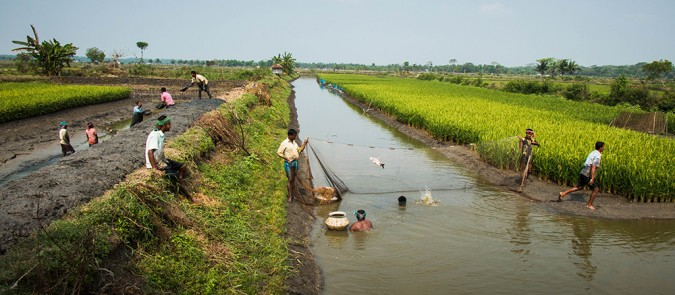
\includegraphics[width=\linewidth]{gher_freshwater.jpg}
    \caption{\textbf{Structure of a Gher in Freshwater Regions :} This image illustrates the layout of a Gher farm in freshwater regions, showing the embankments used to control water levels for fish farming and the deeper channels used for irrigation during the dry season}
    \label{fig:gher_freshwater}
\end{figure}

\begin{figure}[h]
    \centering
    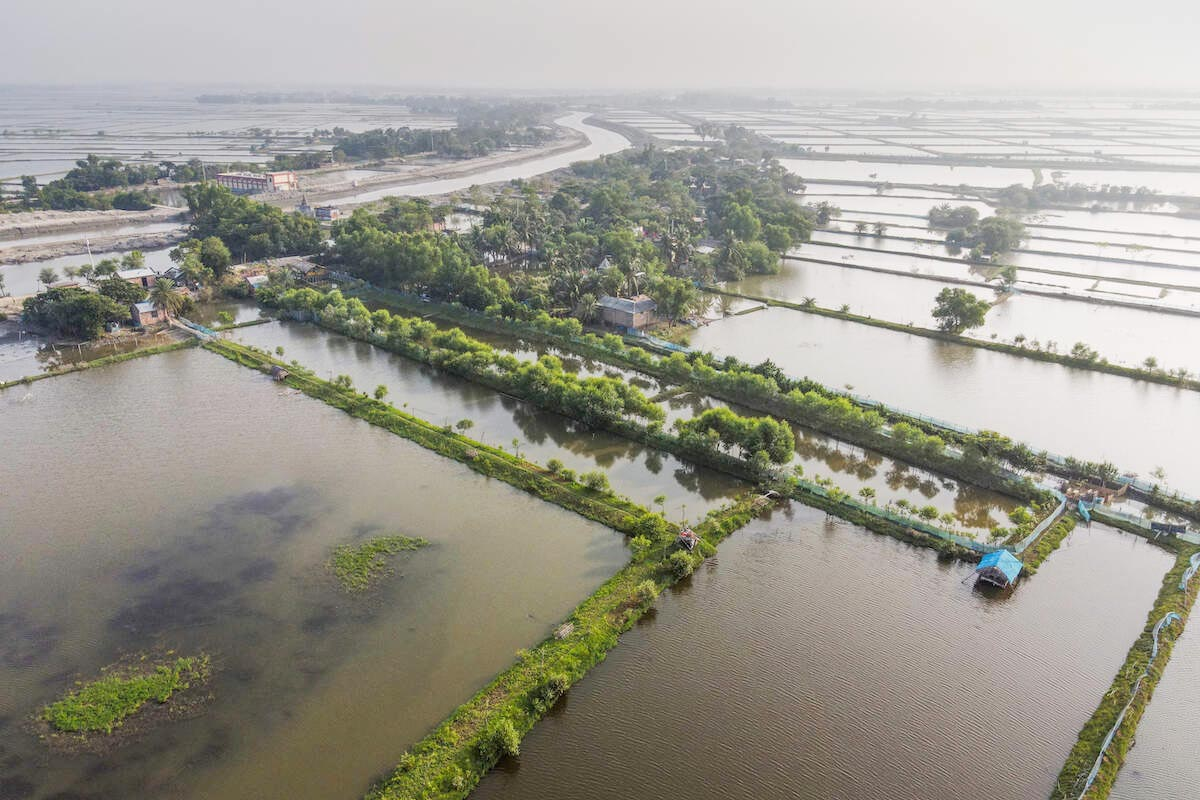
\includegraphics[width=\linewidth]{gher_salty.jpg}
    \caption{\textbf{ Gher Farming in Salty Coastal Regions : } This image provides a view of a Gher farm in a coastal region where shrimp farming is the primary activity during the rainy season, with vegetables being grown on the embankments. }
    \label{fig:gher_salty}
\end{figure}

\begin{figure}[h]
    \centering
    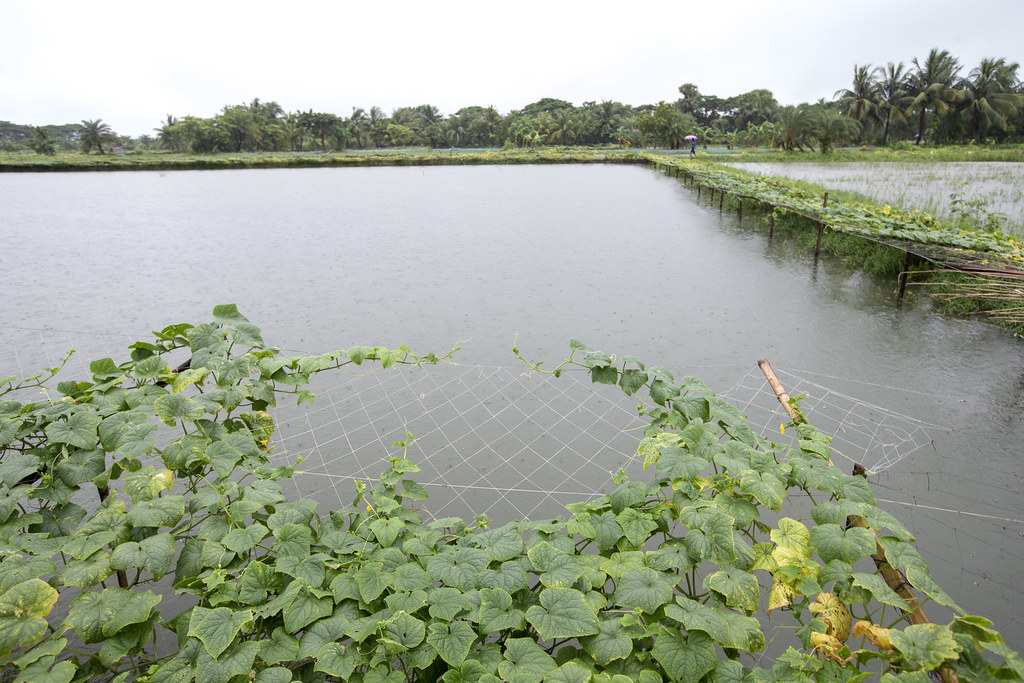
\includegraphics[width=\linewidth]{gher_embankments.jpg}
    \caption{\textbf{Multifunctional Use of Embankments in Gher Farming: } This image highlights the embankments’ role in Gher farming, showing how they are used for both water management and \textbf{vegetable cultivation}, demonstrating the system’s efficiency. }
    \label{fig:gher_embankments}
\end{figure}


\subsection{\textbf{Flood Management in Bangladesh}}
Flooding is a recurrent and increasingly severe issue in Bangladesh, a country particularly vulnerable to the impacts of climate change. Located in the world’s largest delta, Bangladesh's flat, low-lying geography, combined with heavy monsoon rains, makes it prone to seasonal flooding. Over the past few decades, the frequency, intensity, and unpredictability of floods have intensified, largely due to rising global temperatures and sea levels \cite{ref7}. Bangladesh experiences several types of floods—river floods, flash floods, and coastal floods—all of which pose significant challenges to both urban and rural areas. According to the Intergovernmental Panel on Climate Change (IPCC), the impacts of climate change will likely increase the risk of flooding in Bangladesh, making effective flood management and adaptation strategies more critical than ever \cite{ref8}.

Floods in Bangladesh often result in widespread destruction, causing the displacement of millions of people, damage to infrastructure, and loss of agricultural productivity. While the government has implemented various flood control measures, such as embankments and flood forecasting systems, the existing infrastructure remains insufficient to cope with the scale and frequency of modern floods. In many cases, outdated infrastructural systems, such as drainage and embankments, are overwhelmed, leading to ineffective flood mitigation \cite{ref9}. Additionally, organizational challenges during rescue and relief operations exacerbate the impact of flooding. Delays in gathering accurate data on flood-affected areas, coupled with difficulties in coordinating relief efforts, often hinder the effectiveness of flood response operations \cite{ref10}. Given these complexities, there is an urgent need for technological innovation in flood management to improve the real-time response and accuracy of flood mitigation efforts.

One promising solution to these challenges is the development of an autonomous real-time mapping system. Such a system would integrate Unmanned Aerial Vehicles (UAVs) and Unmanned Ground Vehicles (UGVs) to monitor and map flood-affected areas. This dual-purpose system could autonomously create real-time, high-resolution maps of submerged and partially submerged areas, providing critical data to rescue teams and disaster management authorities. With the ability to generate accurate flood maps, response teams could more efficiently allocate resources, identify safe routes, and coordinate rescue efforts. This innovation would address the critical gaps in timely data acquisition and resource allocation, which are key hurdles in Bangladesh’s current flood management framework \cite{ref12}.

Bangladesh is an ideal testing ground for such autonomous systems due to its frequent and diverse exposure to floods. Its unique geographical and climatic conditions make it a high-risk area for flooding, providing ample opportunities for real-world testing of advanced flood management technologies. Moreover, Bangladesh’s history of recurring floods offers a wealth of historical data that can be leveraged to train AI systems and improve the predictive capabilities of mapping technologies. By deploying UAVs and UGVs, autonomous systems could be trained to respond more effectively to the varied topographies and flood dynamics across different regions of the country \cite{ref11}.

In conclusion, the growing threat of flooding in Bangladesh, compounded by infrastructure deficiencies and organizational inefficiencies, calls for innovative solutions in flood management. An autonomous real-time mapping system offers a promising approach to addressing these challenges, enhancing disaster preparedness and response capabilities. By integrating advanced technologies like UAVs and UGVs, such systems could revolutionize flood management not only in Bangladesh but also in other flood-prone regions across the globe.

\subsection{\textbf{Connection Between Floods and Gher Farming}}
The deep relationship between flooding and Gher farming in Bangladesh highlights the vulnerabilities faced by aquaculture and agriculture systems in coastal and freshwater regions. Floods, particularly during the rainy season, have a significant impact on Gher farms, where embankments are essential for maintaining water levels for fish farming. In Bangladesh, flooding significantly affects both urban areas and agricultural systems, including Gher farming. Gher farms, which rely on carefully managed water levels, face substantial risks during the rainy season when floods can damage embankments, cause fish to escape, and contaminate water supplies, leading to severe crop damage and financial losses for farmers \cite{ref5}. The seasonal nature of Gher farming—where fish are farmed during the rainy season and crops are grown on embankments during the dry season—makes these systems particularly vulnerable to overflowing waters, especially in coastal areas where high tides and river floods are common \cite{ref4}.

In coastal areas, where shrimp farming is common, the threat of river floods and tidal surges exacerbates the risk. The combination of high tides and heavy rainfall can easily breach embankments, allowing saline water to enter freshwater farms, contaminating the water and threatening both fish and agricultural production \cite{ref4}. The unpredictable nature of floods, worsened by climate change, makes it increasingly difficult for farmers to prepare and protect their Gher systems from severe damage. As a result, flooding poses a direct threat to the sustainability of Gher farming, leading to long-term economic instability for the communities that depend on it \cite{ref7}.

In addition to these environmental challenges, Gher farms often face threats from fish poisoning and theft. During peace times, malicious acts of poisoning are a frequent issue, often arising from personal or local disputes, where competitors or individuals intentionally introduce toxins into the water to kill fish stocks. Similarly, theft remains a significant concern, as monitoring large Gher areas is challenging, and thieves can exploit weak security to steal fish \cite{ref1}. The monitoring challenge is prevalent for all scales of Gher, from large to small. However, during the rainy season and flood times, fish theft, another significant problem during peacetime, becomes less of a concern during floods. Thieves are unable to access the Gher due to the lack of navigable routes caused by flooding. This natural barrier eliminates the need for active security monitoring during the flood season. Floodwaters dilute any poison, rendering it ineffective, and thieves find it difficult to access Ghers because the routes are submerged, making fish theft less of a concern.

During flood events, UAVs and UGVs can be redirected to focus on flood mapping and emergency monitoring, ensuring that critical water quality issues are detected even in extreme conditions. By repurposing resources for real-time data collection and mapping, these systems can enhance the coordination of flood response efforts, helping to identify safe routes and high-risk areas. Additionally, the data collected during floods can assist farmers in post-flood recovery, providing insights on soil and water conditions that help them prepare better for the upcoming farming season. This makes the integration of Gher farm monitoring and flood management systems a valuable, year-round solution.

\subsection{\textbf{The Need for a Common Solution}}
Given the critical challenges posed by floods to both Gher farming and broader flood management, there is a strong need for a multi-purpose system that integrates agricultural monitoring with flood disaster response. A dual-purpose autonomous system utilizing technologies such as Unmanned Aerial Vehicles (UAVs), Unmanned Ground Vehicles (UGVs), AI, IoT, and sonar technology can effectively address these needs. This system would serve as a comprehensive solution for both peace-time monitoring and emergency flood management, providing continuous value throughout the year.


During peace times, the system would primarily focus on monitoring water quality in Gher farms, ensuring that contamination from environmental pollutants or intentional acts of poisoning is detected early. By using IoT sensors and AI-based analysis, the system can provide real-time alerts to farmers, enabling them to take prompt action before water quality issues escalate. Additionally, UGVs and UAVs can patrol the Gher farms, preventing theft by monitoring for suspicious activity, thus reducing fish losses from both theft and environmental hazards. The sonar technology embedded in UGVs can continuously track fish health, movement patterns, and water quality, while IoT sensors provide farmers with live updates on the conditions of their Gher farms \cite{ref1}, \cite{ref6}.


In emergency situations, such as during flood events, the role of the system shifts. As fish theft and poisoning are less of a concern during floods, the system can be repurposed for flood disaster response. UAVs and UGVs can be redirected to focus on real-time flood mapping and emergency monitoring, providing accurate data on submerged areas, safe routes, and high-risk zones. This real-time information would be crucial for rescue teams, enhancing the coordination and efficiency of flood response efforts and ensuring that resources are allocated effectively, helping to save lives and protect properties \cite{ref7}, \cite{ref10}. By repurposing existing resources during floods, this system maximizes its utility, making it a cost-effective solution for addressing both agricultural security and disaster management.


The dual-purpose functionality of this integrated system offers significant cost-efficiency by ensuring that the technology is utilized for year-round operations. During peace times, it would enhance agricultural productivity and security by monitoring water quality and preventing theft, providing farmers with the tools to manage their farms more effectively. During flood events, the system would contribute to disaster management by providing accurate, real-time mapping and monitoring that can guide emergency response teams. This versatility makes the system particularly valuable for regions where flooding is a frequent challenge, such as Bangladesh, which provides an ideal environment for developing and testing the system due to its regular exposure to floods. However, the same integrated solution can be implemented in other flood-prone areas globally, making it adaptable to diverse geographical and climatic conditions \cite{ref5}, \cite{ref9}.


During flood events, the real-time maps generated by the system will be publicly accessible, similar to Google Maps, enabling relief and rescue teams to navigate affected areas more effectively. This open access will also allow relatives of people in flood-affected zones to stay informed about the conditions, facilitating communication and safety planning. Furthermore, the availability of up-to-date maps will aid various social organizations that conduct rescue missions during floods, making their efforts more efficient and coordinated. By addressing the needs of Gher farming and flood management within a single system, this approach offers a scalable, cost-effective solution that can benefit farmers, disaster response teams, and communities across different regions \cite{ref12}, \cite{ref13}.



\section{\textbf{Literature Review}}

As the challenges posed by \textit{climate change} and \textit{frequent flooding} become more pronounced, autonomous systems such as \textbf{Unmanned Aerial Vehicles (UAVs)} and \textbf{Unmanned Ground Vehicles (UGVs)} have gained attention as tools for addressing both \textit{agricultural monitoring} and \textit{flood management}. This literature review explores the current advancements in \textbf{UAV} and \textbf{UGV} technologies, with a focus on their role in \textit{disaster response} and \textit{agricultural security}, particularly for Gher farming in flood-prone areas like Bangladesh.

While \textbf{UGVs} are the primary focus of this review, part of this research will explore whether other vehicle types, such as \textbf{Amphibious Ground Vehicles (AGVs)} or vehicles designed to float in flooded conditions, may offer additional benefits. The project will aim to determine which vehicle type is best suited for \textit{dual-purpose operations}, ensuring the system is capable of monitoring \textbf{Gher farms} during \textit{peace times} and providing \textit{real-time flood mapping} in emergency situations.

The literature review is divided into two primary sections, reflecting the dual focus of this research on Gher farming systems and flood management systems. These sections provide a comprehensive overview of existing technologies and methods relevant to both agricultural monitoring and flood response.

\textbf{A. Gher Farming Systems}
This section examines the existing practices and technologies used in Gher farming, including \textit{water quality monitoring}, \textit{theft prevention}, and \textit{contamination control}. A significant concern in Gher farming is the intentional \textit{poisoning} of water bodies, which can result in large-scale losses of fish and shrimp. The review highlights preventive strategies and technological solutions aimed at minimizing this risk. Emerging technologies, such as \textit{Internet of Things (IoT)} sensors and \textit{autonomous systems}, are explored for their potential in improving farm management, productivity, and response to poisoning incidents.

\textbf{B. Flood Management Systems}
This section reviews modern flood management techniques, focusing on \textit{real-time flood monitoring}, \textit{AI-driven flood prediction}, and the application of \textit{autonomous systems}, such as \textbf{Unmanned Aerial Vehicles (UAVs)} and \textbf{Unmanned Ground Vehicles (UGVs)}, for disaster response. It covers both \textit{traditional} and \textit{technological} approaches to managing floods, particularly in regions like Bangladesh.

These sections collectively provide the necessary background on existing systems related to both Gher farming and flood management, offering a foundation for the proposed integrated solution.



\subsection{\textbf{Gher Farming Systems}}
\begin{enumerate}
	\item \textbf{AI-Driven Sonar-Based Monitoring Systems in Aquaculture : }
	
Sonar technology has been widely used in aquaculture to monitor fish movement, population density, and biomass estimation. It has been demonstrated how sonar technology can help farmers monitor fish populations and track movement patterns in real-time, leading to more informed decision-making for aquaculture management \cite{ref13}. However, research on integrating AI algorithms with sonar systems for detecting underwater threats, such as hidden nets or traps, remains limited.

AI-driven sonar systems offer significant potential for detecting underwater security threats. Large-scale farms may face challenges with monitoring vast water bodies, while smaller farms may not have the financial resources for advanced systems. The need for scalable and cost-effective solutions that can cater to the diverse needs of different farm sizes has been highlighted \cite{ref14}. The development of AI-driven sonar technology could provide a versatile solution that can be adapted to various farm sizes, allowing farmers to detect and respond to underwater threats more effectively.


	\item \textbf{IoT-Based Water Quality Monitoring in Aquaculture}
	
	Water quality is critical for the health and sustainability of aquatic species in aquaculture, regardless of the size of the farm. Monitoring parameters such as pH, dissolved oxygen, ammonia levels, and toxic substances is essential for maintaining the optimal health of fish populations \cite{ref7}.

IoT-based water quality monitoring systems have become increasingly popular in aquaculture, enabling farmers to continuously track water quality and respond to changes in real-time. The potential of IoT sensors for monitoring water quality in Bangladeshi aquaculture has been explored, demonstrating the effectiveness of real-time alerts in preventing contamination and poisoning incidents \cite{ref16}. However, most existing systems are focused on monitoring basic water quality parameters and do not incorporate predictive analytics or early warning systems to detect poisoning or contamination events.

In Gher farming, where water quality can vary significantly across different sections, establishing a centralized water analysis center could enhance monitoring capabilities \cite{ref17}. The potential for IoT sensors to feed into such a central system could provide real-time, location-specific insights, ensuring optimal water conditions for both fish farming and paddy cultivation \cite{ref18}.

	\item \textbf{Autonomous Robotic Systems for Contamination Control and Flood Management in Aquaculture: }
	Autonomous robotic systems have gained traction in the field of aquaculture for tasks such as water monitoring, fish feeding, and sample collection. Autonomous Surface Vehicles (ASVs) have been used in aquaculture, demonstrating their ability to navigate water bodies and perform tasks such as distributing nutrients evenly across a pond \cite{ref19}. However, there is limited research on the use of these vehicles for contamination control and flood management.

Flooding poses a significant threat to aquaculture, particularly in flood-prone regions. While there has been substantial research on flood management systems in urban areas \cite{ref20}, the application of autonomous systems for managing floodwaters and contamination in aquaculture remains largely unexplored. Autonomous robotic systems capable of deploying barriers or isolating contaminated areas in response to real-time sensor data could help farms mitigate the impact of flooding and contamination on their operations, making it highly relevant for both small and large-scale operations.

While ASVs have been investigated for water quality monitoring \cite{ref19}, the use of robotics for emergency situations such as preventing fish escapes during water overflows has not been fully explored. The potential for robots in handling various aquaculture tasks has been discussed, but using robots to automatically deploy blue net fences during overflow events is a novel approach. This could prevent fish from moving between Ghers during heavy rainfall, significantly reducing losses in flood-prone regions \cite{ref21}.

\item \textbf{AI-Powered Decision Support Systems for Theft Prevention: }

Fish theft is a major concern for aquaculture farms, particularly for large-scale operations with extensive water bodies that are difficult to monitor. The potential of machine learning to detect unusual patterns in fish movement that may indicate theft or unauthorized activity has been explored \cite{ref22}. However, the current application of machine learning in aquaculture theft prevention remains limited, with most farms relying on manual inspections or camera-based systems that require constant human intervention.

AI and machine learning systems could analyze real-time data from sonar and IoT sensors, developing predictive models to detect suspicious activities such as unusual fish movement patterns. Such AI-powered decision support systems could provide actionable insights for farm managers, helping them prevent theft and protect their assets. By combining data from multiple sources (sonar, IoT, cameras), the system would offer comprehensive monitoring that can be scaled for both small and large farms.

\item \textbf{Integrated Technological Solutions for All-Scale Aquaculture : }

While much of the existing literature has focused on large-scale aquaculture technologies, smaller operations have often been underserved by advanced technological solutions due to cost and complexity. The growing need for scalable and affordable technologies that can cater to both small and large-scale farms has been highlighted \cite{ref15}. As climate change continues to pose challenges for aquaculture, including more frequent and severe flooding events, the need for resilient, integrated technological solutions becomes even more critical.

Modular, scalable solutions that combine AI, IoT, sonar technology, and robotics for both small-scale and large-scale farms can improve security and water quality management. The use of autonomous robotic features could also enhance farm resilience to climate-related risks such as flooding. This approach ensures that farmers, regardless of their farm size, can benefit from cutting-edge technologies that are both affordable and adaptable.

Additionally, water overflow management through automated systems remains underexplored in current literature. Traditional and automated methods for managing aquaculture systems have been identified \cite{ref23}, \cite{ref24}, but research has not yet addressed the challenge of fish escape during floods using robotically deployed barriers. Incorporating such systems could provide significant benefits for Gher farming, enhancing both resilience and operational efficiency.

\end{enumerate}





\subsection{ \textbf{Flood Management Systems}}
Flood management systems have evolved significantly over the years, integrating advanced technologies to enhance preparedness, response, and recovery efforts. These systems are crucial for protecting both urban infrastructure and rural agricultural practices like Gher farming, especially in flood-prone regions such as Bangladesh.
\begin{enumerate}

\item \textbf{ Traditional Flood Management Techniques :}
Historically, flood management has relied on structural interventions, including embankments, levees, and flood walls, to prevent floodwaters from inundating vulnerable areas. While these systems provide some level of protection, they are often reactive in nature and require significant maintenance. In regions with recurring floods, such as Bangladesh, these structures alone are insufficient to manage increasingly severe and unpredictable weather events \cite{ref9}.

\item \textbf{ IoT-Based Flood Monitoring and Early Warning Systems : }
With the rise of IoT technologies, flood management has seen a shift towards real-time monitoring and data-driven early warning systems. IoT sensors can be deployed in flood-prone areas to monitor water levels, rainfall, and river flows continuously. These sensors relay real-time data to centralized systems, enabling authorities to issue timely flood warnings. Research shows that in countries like Bangladesh, IoT-based flood monitoring systems significantly enhance disaster preparedness and early response, reducing potential damage to both infrastructure and agriculture \cite{ref10}, \cite{ref11}.

\item \textbf{AI and Predictive Analytics for Flood Risk Management: }
Artificial Intelligence (AI) and predictive analytics have emerged as powerful tools in flood risk forecasting. By analyzing historical flood data alongside real-time inputs from IoT sensors, AI models can predict flood events with greater accuracy. These predictive models enable proactive measures, such as evacuations and the deployment of emergency resources, ahead of flood events \cite{ref12}. AI-driven flood management systems are currently being deployed in several flood-prone regions, where they have improved response times and resource allocation.

\item \textbf{Autonomous Systems for Flood Response: }
The introduction of autonomous systems, such as UAVs and UGVs, has further enhanced flood management efforts. UAVs are used for aerial surveys of flood-affected areas, providing high-resolution images that assist in rescue and relief operations. In parallel, UGVs can navigate flooded environments to assess damages and identify safe zones for evacuation. These autonomous systems are particularly effective in areas where human intervention is dangerous or impractical. By integrating UAVs and UGVs with IoT flood monitoring systems, flood response can become faster and more coordinated \cite{ref13}, \cite{ref14}.

\item \textbf{Integrated Flood Management Solutions : }
In many regions, modern flood management systems combine multiple technologies—IoT sensors, AI predictive models, and autonomous systems—to create comprehensive, multi-layered flood management strategies. These integrated systems not only provide real-time monitoring and early warnings but also support disaster response efforts with real-time mapping and autonomous intervention. Countries with frequent and severe floods, like Bangladesh, are increasingly adopting these systems to mitigate the impact of floods on both urban and rural environments \cite{ref15}.

\end{enumerate}



\section{\textbf{Research Gaps}}
Despite significant advancements in the use of autonomous systems for both Gher farming and flood management, several critical gaps remain unaddressed in the existing literature. In the context of Gher farming, current technologies such as IoT sensors and robotics are primarily adopted by large-scale operations, while small to medium-sized farms lack access to affordable, scalable solutions. Key challenges, including water overflow management, contamination control, and theft prevention, remain inadequately addressed. Moreover, the intentional poisoning of Gher water bodies, a critical issue for many farmers, has not yet seen the development of effective preventive solutions, leaving farms vulnerable to catastrophic losses.

Similarly, in the field of flood management, there is limited research on the coordination between UAVs and Amphibious UGVs for real-time flood response. While sonar-based 3D mapping technology has advanced, its use in flooded terrains remains underutilized, and the autonomy of UAV-UGV systems is constrained by current limitations in battery management. Furthermore, there is a growing need for cost-effective, dual-purpose systems that can address both disaster response and agricultural monitoring in a scalable manner.


This research aims to address these gaps by developing an integrated system that combines AI, IoT, UAVs, and UGVs for year-round agricultural and disaster management operations, including potential solutions for intentional poisoning prevention.

\subsection{ \textbf{Gaps in Gher Farming and Aquaculture Technologies}}
\begin{enumerate}
	\item \textbf{ Lack of Automated Systems for Water Overflow Management : }
	While studies have explored manual methods and traditional barrier systems for controlling water overflow in aquaculture \cite{ref23}, the literature reveals a gap in the development of automated systems for managing water overflow, particularly in Gher farming. Current research on automation in aquaculture \cite{ref24} primarily focuses on feeding systems and water quality monitoring, leaving a clear gap in addressing the need for automated solutions that can respond to rising water levels during heavy rainfall or floods, especially for preventing fish escapes.
	
	\item \textbf{ Limited Adoption of Centralized Water Quality Monitoring in Gher Farming : }
	Although centralized water quality monitoring systems have been successfully adopted in large-scale aquaculture \cite{ref17}, there is minimal research on their use in small to medium-sized operations like Gher farming. The literature often discusses IoT-based water quality sensors \cite{ref18} but does not address how these sensors could be integrated into a centralized system for comprehensive water analysis across different sections of the  Gher. This represents a significant gap, as centralized monitoring could improve water quality management and early detection of issues like contamination or pollution.
	
	\item \textbf{Underexplored Use of Robotics for Contamination Control : }
	Robotics has gained attention in aquaculture for routine tasks such as fish feeding and monitoring \cite{ref19}, but the literature lacks studies on robotics for contamination control and flood management in Gher farming. While emergency response systems using robotics have been explored \cite{ref21}, there is limited focus on their use in managing contamination in Gher environments, particularly in response to water contamination or overflow events that could harm fish or shrimp populations.
	
	\item \textbf{ Insufficient Focus on AI-Powered Theft Prevention Systems in Gher Farming : }
Current research on AI and machine learning for aquaculture theft prevention \cite{ref22} has been largely focused on large-scale farms. The literature provides few examples of how these systems could be applied to Gher farming, where fish monitoring can be particularly challenging due to the vast size of the water bodies. Traditional manual monitoring and camera-based surveillance are labor-intensive and have limitations, but there is a lack of research on how AI could enhance theft prevention specifically for Gher farms.
	
	\item \textbf{Lack of Scalable and Affordable Technology for Small to Medium-Scale Gher Farming: }
Technological advancements in aquaculture tend to focus on large-scale, commercial operations \cite{ref15}, leaving small to medium-sized Gher farms underserved by affordable, scalable solutions. The literature points to significant barriers in the adoption of advanced technologies in smaller farms due to cost and complexity, but there is minimal research on developing modular, affordable solutions that could be adapted to smaller farms. This gap highlights the need for scalable technologies that can be implemented incrementally based on the resources and needs of individual Gher farms.
\end{enumerate}

\subsection{\textbf{Gaps in UAV and UGV Coordination for Flood Management}}
\begin{enumerate}
    \item \textbf{ Lack of Research on UAV and Amphibious UGV Coordination for Flood Management : }
Existing studies (e.g., \cite{ref20}, \cite{ref22}) have explored UAVs and UGVs for disaster management independently, but few have focused on their integrated use in flood-affected areas, especially with regard to amphibious UGVs. The challenge of mapping submerged and dry roads in flood zones remains underexplored. Most studies on UAVs focus on aerial data collection, while UGVs are often limited to ground-based operations on dry land. There is little research on cooperative systems where UAVs provide real-time aerial data and guide amphibious UGVs, which are equipped with sonar, to map submerged terrains. This gap indicates a lack of real-time, comprehensive flood terrain mapping systems that combine both aerial and ground-level data.
  
	\item \textbf{ Limited Use of Sonar Technology for Real-Time Mapping of Submerged Terrains : }
	Although sonar technology is used in military and environmental monitoring, there is minimal research on its application in civilian disaster management, particularly for real-time mapping of submerged roads during floods. Current disaster management literature does not fully address how sonar-equipped UGVs can be used to navigate and assess underwater terrain (e.g., \cite{ref13}, \cite{ref14}). The proposed system addresses this by integrating sonar technology into UGVs to provide 3D maps of submerged areas, allowing for more detailed and accurate assessments of flood-affected roads, a capability that has been overlooked in previous studies.

	
	\item \textbf{ Need for Improved Autonomy and Battery Management in UAV-UGV Systems : }
While autonomous systems are a focus of much disaster management research, existing studies (e.g., \cite{ref21}) have not sufficiently explored autonomous battery management for UAV-UGV systems in flood zones. The literature does not address how UAVs can autonomously recharge UGV batteries, thus enabling prolonged, uninterrupted operations. The proposed system introduces a novel battery-swapping functionality where UAVs autonomously extend UGV operational time, allowing for long-distance and long-duration operations with minimal human intervention. This is a critical gap in current research, which primarily focuses on human-operated or semi-autonomous systems.
	
	
	\item \textbf{Cost-Efficiency and Long-Term Utility of Dual-Purpose Systems : }
	Research has highlighted the importance of cost-efficiency in autonomous systems (e.g., \cite{ref23}, \cite{ref24}), but there is a lack of focus on dual-purpose technology that can be used both during crises and in non-crisis times. Most autonomous systems are designed for single-use, disaster-specific operations, which leads to high costs and underutilization during non-emergency periods. The proposed system addresses this gap by ensuring year-round usage of UGVs through their deployment for Gher farming security and environmental monitoring in agricultural settings. This dual-purpose functionality increases the return on investment and prevents system degradation, offering a solution to the cost-efficiency challenges not discussed in the existing literature.
	
	\item \textbf{Inadequate Real-Time and Dynamic Mapping Systems in Disaster Scenarios : }
Most current mapping systems in disaster management (e.g., \cite{ref17}, \cite{ref18}) are static and do not adapt to the rapidly changing conditions in flood zones. While these systems provide valuable data, they fail to offer dynamic updates that reflect real-time changes in submerged and dry terrains. The proposed system fills this gap by providing real-time, continuously updated maps via a web-based platform, ensuring that rescue teams always have access to the most accurate and current terrain data. This real-time adaptability is crucial for improving the effectiveness of disaster response, but it remains underexplored in current research.
		
\end{enumerate}	


\section{\textbf{Proposed Solution}}

\subsection{\textbf{Integrated AI, IoT, and Robotics Systems for Gher Farming Security and Water Quality Management}}
\begin{enumerate}
	\item \textbf{AI-Driven Sonar-Based Monitoring System for Threat Detection : }
In Gher farming, particularly during the rainy season, water levels often fluctuate, making it challenging to monitor fish movement and prevent theft or fish escapes. The proposed system will implement an AI-driven sonar system to monitor underwater activities in real-time. This system leverages sonar technology to detect threats such as hidden nets or traps used for fish theft, as well as sudden changes in fish behavior due to environmental stressors.
The system will continuously scan the Gher, analyzing fish movement patterns and detecting anomalies that could indicate potential threats. AI algorithms will establish a baseline of normal fish behavior, and deviations 

from this norm (such as irregular fish activity) will trigger alerts to the farmer for immediate intervention \cite{ref13}, \cite{ref14}. This scalable solution can be adapted to both small-scale Ghers and large-scale aquaculture systems, offering versatility in application across different sizes of farming operations.
	
	\item \textbf{IoT-Based Centralized Water Quality Monitoring and Early Warning System : }
	Maintaining optimal water quality is critical for the success of Gher farming, particularly during both the rainy and dry seasons. The proposed system includes an IoT-based centralized water analysis center, which will monitor key water parameters such as pH, dissolved oxygen, ammonia levels, and toxic substances.
	
IoT sensors will be deployed throughout different sections of the Gher, continuously collecting data and transmitting it to a central hub where the water quality across the entire farm can be analyzed \cite{ref18}. The central water analysis center will aggregate this data to provide comprehensive insights into water quality variations, ensuring that any harmful changes are detected early and that the water conditions remain suitable for fish or shrimp farming \cite{ref17}. AI-based predictive models will analyze historical data to forecast potential contamination or poisoning events before they occur. When abnormalities are detected, real-time alerts will be sent to the farmer via mobile devices or a web-based platform, ensuring rapid response to mitigate risks.


	\item \textbf{Autonomous Robotic System for Water Overflow and Contamination Control : }
	Heavy rainfall during the monsoon season can cause water to overflow the embankments or dikes in Gher farms, leading to the escape of fish into neighboring Ghers or other bodies of water. Traditionally, farmers set up blue net fences to prevent such escapes, but this is often difficult to execute quickly, especially during nighttime rainfalls.
	
The proposed system will incorporate robots that automatically deploy blue net fences around the Gher in response to rising water levels, ensuring that the fish remain contained within the designated areas \cite{ref21}. These robots will be activated based on real-time data from water level sensors, reducing the need for human intervention during overflow events. Additionally, these autonomous robotic systems will be equipped to handle contamination control. In the event of water contamination detected by the IoT sensors, the robots will deploy containment barriers to isolate the affected section of the Gher, preventing the spread of toxins to the rest of the farm \cite{ref19}. This autonomous emergency response system significantly reduces the risk of fish loss during floods and ensures that water contamination is managed swiftly and effectively.
	
	
	\item \textbf{ AI-Powered Decision Support System for Theft Prevention : }
Fish theft remains a significant issue in Gher farming, particularly in large ponds and ponds located in distant areas that are difficult to monitor. The proposed system integrates AI-powered decision support tools to predict and prevent theft by analyzing real-time data from sonar, IoT sensors, and cameras.

Machine learning models will identify unusual patterns in fish movement that may indicate theft, providing early warnings to farm operators \cite{ref22}. The decision support system will also provide actionable insights on how to adjust fish stocking patterns or increase surveillance in areas more prone to theft. This data-driven approach ensures that farm security is proactive rather than reactive.
	
	
	\item \textbf{ Scalable, Affordable Solutions for Gher Farming : }
One of the key strengths of this system is its scalability and affordability. The modular design allows it to be adapted for small-scale Gher farms as well as large industrial operations, ensuring that farms of all sizes can benefit from advanced aquaculture technologies. Low-cost IoT sensors and open-source AI algorithms will ensure that even small farmers can afford to implement key components of the system. Larger operations can scale up by integrating additional features such as autonomous robots and centralized water monitoring systems \cite{ref18}. The modular architecture of the system allows for customized deployment, enabling each farm to implement the components most suited to their specific needs and environmental challenges.
	
	
	\item \textbf{Resilience to Climate Challenges : }
	The system is designed to enhance the climate resilience of Gher farms, particularly in flood-prone regions. The robotically deployed blue net fences and water containment barriers will ensure that fish are protected during periods of heavy rainfall, while the centralized water quality monitoring system will help farms quickly respond to environmental changes caused by extreme weather \cite{ref23}, \cite{ref24}. By addressing these challenges, the system promotes sustainable farming practices that help protect both the environment and the farmer’s livelihood, even in the face of climate-induced challenges like floods.
	
\end{enumerate}


\subsection{\textbf{Autonomous UAV and UGV System for Flood Management and Agricultural Security}}
To address the gaps identified in the existing literature, this research proposes a highly autonomous system that integrates Unmanned Aerial Vehicles (UAVs) and Unmanned Ground Vehicles (UGVs) for the dual purposes of flood management and agricultural monitoring. This system leverages the aerial reconnaissance capabilities of UAVs and the amphibious, sonar-equipped UGVs for submerged and ground-level terrain mapping. It is designed to deliver real-time, detailed mapping of flood-affected areas and offers long-term utility for agricultural monitoring during non-flood periods, addressing key needs in both areas \cite{ref1}–\cite{ref3}.
\begin{enumerate}
	\item \textbf{UAV and UGV Cooperative System for Real-Time Mapping : }
	The core innovation of the proposed system is the integration of UAVs and UGVs for high-precision, real-time mapping of both submerged and dry roads in flood-prone areas. UAVs provide aerial reconnaissance, capturing data from above, including flood zones, obstacles, and safe routes, which is transmitted to the ground control center and UGVs for immediate action \cite{ref4}. The amphibious UGVs, equipped with sonar technology, are responsible for mapping submerged roads and detecting underwater obstacles, guided by UAVs to critical locations. This UAV-UGV collaboration enhances the precision and efficiency of flood mapping by including underwater terrain assessments, a capability missing from most existing flood management systems \cite{ref5}.
	
	\item \textbf{Sonar-Based 3D Terrain Mapping : }
Amphibious UGVs use advanced sonar sensors to create 3D maps of submerged areas, identifying debris, broken roads, and other underwater hazards. These UGVs can operate in both water and land environments, allowing them to navigate regions where traditional vehicles would fail \cite{ref6}. The sonar-generated 3D maps provide real-time updates and give rescue teams an accurate, dynamic understanding of submerged road conditions, which is critical for safe navigation and rescue operations \cite{ref7}.
	
	\item \textbf{Autonomous Battery Management for Extended Operations : }The system introduces battery-swapping functionality between UAVs and UGVs, supporting long-duration, long-distance operations with minimal human intervention. UAVs not only provide aerial surveillance but autonomously recharge UGVs' batteries, allowing them to operate continuously for extended periods. This feature addresses limitations in current systems that require frequent human intervention for battery management \cite{ref8}. Extended battery life increases the range and efficiency of the system, enabling continuous operation during crucial disaster situations \cite{ref9}.
	
	
	\item \textbf{Web-Based Real-Time Map Access : }
To enhance relief operations, the system provides real-time map updates accessible via a web platform. These maps reflect the latest flood conditions, submerged roads, and hazards, with clearly marked safe routes, damaged roads, and obstacles, aiding rescue teams in planning efficient operations \cite{ref10}. Continuous updates address the gap in static mapping systems and ensure that rescue operations are based on current information \cite{ref11}.
	
	\item \textbf{Dual-Purpose Functionality for Agricultural Monitoring:}
To maximize cost-efficiency and long-term utility, UGVs are repurposed for Gher farming and agricultural monitoring during non-disaster periods. This dual-purpose functionality keeps UGVs active throughout the year, preventing system degradation due to inactivity and ensuring a high return on investment \cite{ref12}. The amphibious UGVs can patrol both land and water in Gher farms, providing security and monitoring for optimal farming conditions \cite{ref13}. This dual-purpose capability offers an innovative use case, especially where single-purpose deployments are less sustainable \cite{ref14}.
	
\end{enumerate}


\subsection{\textbf{Expected Contributions of the Proposed System}}
The proposed autonomous UAV and UGV system addresses critical gaps in current flood management and agricultural monitoring. By combining aerial and sonar-based mapping, the system delivers real-time, detailed terrain assessments in flood-affected areas, enhancing disaster response efficiency. The autonomous battery-swapping functionality and dual-purpose agricultural applications contribute to the system’s cost-effectiveness and operational sustainability. This solution not only improves disaster management but also ensures continuous value through agricultural security, making it a versatile technology for flood-prone regions.

\begin{enumerate}
	\item \textbf{Improved Disaster Response Efficiency: } 
	By enabling UAV-UGV coordinated mapping, the system will improve rescue teams' ability to navigate flood-affected areas. The integration of sonar-equipped UGVs will ensure detailed 3D mapping of underwater terrains, providing data beyond what aerial reconnaissance alone can achieve \cite{ref3}.

	\item \textbf{Extended Operational Range with Minimal Human Intervention :}
The autonomous battery-swapping feature extends the operational range of UGVs, allowing long-distance, long-duration operations in flood zones with reduced human involvement. This innovation enhances continuous operation during critical disaster periods \cite{ref4}.
	
	\item \textbf{Year-Round Cost-Efficiency : }
The system’s dual-purpose design, where UGVs are repurposed for agricultural monitoring in non-disaster times, ensures that technology remains in active use throughout the year. This feature offers significant cost-efficiency and prevents the degradation associated with seasonal-only deployments \cite{ref6}.
	
	\item \textbf{Accurate, Dynamic Mapping for Relief Teams : }
By providing real-time, accessible map updates through a web platform, the system enables relief teams to plan and execute operations based on the most current data. This dynamic capability directly addresses the shortcomings of static maps, which may quickly become outdated during emergencies \cite{ref7}.
		
\end{enumerate}


\section{\textbf{Future Development and Global Applicability}}
The proposed dual-purpose autonomous system, while initially designed for Gher farming and flood management in Bangladesh, holds significant potential for broader applications in various flood-prone regions and aquaculture practices worldwide. Additionally, the system can be further developed to address critical needs in road safety monitoring and emergency medical supply delivery, both in peace and emergency times. The scalability of this system, coupled with its adaptability to other applications, makes it a valuable tool for enhancing public safety, aquaculture resilience, and disaster management globally.

\begin{enumerate}
	\item \textbf{Adaptability to Various Aquaculture and Environmental Systems :}
Global aquaculture systems face numerous challenges, including environmental contamination, theft prevention, and the need for continuous water quality monitoring. Studies demonstrate that regions with similar aquaculture practices to Gher farming, such as parts of Southeast Asia, Africa, and the United States, would benefit from systems ensuring real-time monitoring and automated responses to environmental changes. For instance, IoT-based sensors and AI systems have proven effective in managing water quality and improving the resilience of aquaculture in these areas, though they often lack an integrated approach \cite{ref25}, \cite{ref26}. IoT and AI-driven monitoring systems have shown significant potential in providing continuous feedback on environmental conditions, allowing for early intervention to prevent losses due to contamination or theft \cite{ref27}. By configuring the technology to meet local environmental requirements, the proposed system could be adapted to support different aquaculture practices and varying environmental needs, making it relevant to a broader range of aquaculture systems \cite{ref28}.
	
	\item \textbf{ Global Applications for Flood Management:}
	Flood management remains a critical challenge worldwide, with frequent floods affecting urban and rural areas in countries like Brazil, India, and the United States. Existing flood management solutions have incorporated autonomous systems, including UAVs and UGVs, to monitor water levels and predict flood risks; however, there is still a significant gap in real-time flood mapping using coordinated UAV-UGV systems. Research highlights the need for real-time mapping solutions in flood-prone areas to support rapid response and efficient resource allocation \cite{ref29}, \cite{ref30}. Integrating amphibious UGVs with UAVs for coordinated flood mapping, as proposed in this study, would provide immediate situational awareness and actionable data for emergency response teams. This application can extend beyond Bangladesh, assisting disaster management teams in Latin America, Asia, and Europe, where similar challenges arise \cite{ref31}.
	
	
	\item \textbf{Potential for Road Safety Monitoring and Emergency Medical Response : }
	In peaceful times, the proposed system can support public safety through autonomous road monitoring and emergency response. Drones equipped with cameras and sensors can autonomously respond to traffic accidents, providing on-the-ground reconnaissance and assessing accident severity, enabling rapid and informed emergency responses. Studies show that drones can play a significant role in improving response times to incidents in remote or congested areas, reducing fatalities and supporting public safety initiatives \cite{ref32}. Additionally, drones can be employed in emergency medical supply delivery to remote locations lacking immediate healthcare access. This capability has been implemented on a limited scale by some e-commerce companies, but a dual-purpose, comprehensive system integrating flood mapping, road safety monitoring, and emergency medical delivery has yet to be explored \cite{ref33}, \cite{ref34}. Establishing numerous drone stations would facilitate quick dispatch of drones for medical emergencies, accident response, or flood events, maximizing the system’s utility year-round.
	
	
	\item \textbf{Need for Regulatory Framework and Operational Guidelines : }
	To implement a dual-purpose autonomous system effectively, a comprehensive regulatory framework governing drone operations is essential. Literature on drone regulation highlights gaps in current frameworks, especially regarding airspace management, privacy concerns, and the integration of UAVs and UGVs in public spaces \cite{ref35}. For a system addressing both agricultural and disaster management needs, several regulatory considerations are essential:
	\begin{enumerate}
		\item \textbf{Operational Authority : } Identify the governing body responsible for overseeing dual-purpose drones and establishing deployment protocols.
		\item \textbf{Data Privacy and Security:}Define standards for securely storing and managing data, ensuring public privacy while facilitating real-time monitoring.
		\item \textbf{Airspace Management:} Establish clear guidelines for flight paths, altitude restrictions, and response protocols to minimize conflicts with other aerial systems.
		\item \textbf{Network-Based Management:} Develop a centralized drone management network enabling real-time communication, command issuance, and efficient resource coordination across multiple drone stations \cite{ref36}.
	\end{enumerate}
\end{enumerate}
By addressing these regulatory needs, the system could be safely and effectively integrated into public infrastructure, supporting emergency response, flood mapping, and aquaculture monitoring.
The proposed dual-purpose system is designed with adaptability and scalability, allowing it to expand beyond its initial focus on Gher farming and flood management in Bangladesh. By customizing the system for global aquaculture practices and implementing additional applications like road safety monitoring and emergency medical supply delivery, this solution could benefit a broad spectrum of public safety, agricultural, and disaster management initiatives. Furthermore, establishing a comprehensive regulatory framework is critical to ensure safe, ethical, and efficient operation across diverse applications. This forward-looking approach not only strengthens the utility of the system but also positions it as a model for multi-functional autonomous systems applicable across flood-prone and rural communities worldwide.


\section{\textbf{Problem Statement}}
In flood-prone regions worldwide, aquaculture systems and public safety infrastructure face substantial challenges due to the increasing impacts of climate change and extreme weather events. Practices like Gher farming in Bangladesh and other aquaculture systems across Southeast Asia, Africa, and Latin America are highly vulnerable to environmental degradation, theft, and intentional contamination. These challenges, along with the absence of affordable and scalable monitoring solutions, threaten the economic stability of small to large-sized fish farms and exacerbate food security concerns.

Flood management infrastructure in these areas is similarly insufficient to handle the real-time demands of dynamic flood events. Conventional systems lack the capability for real-time data collection and response, creating critical gaps in disaster preparedness and resource allocation during emergencies. While autonomous systems, such as Unmanned Aerial Vehicles (UAVs) and Unmanned Ground Vehicles (UGVs), have been applied individually in agriculture or flood response, there is a gap in developing a comprehensive, dual-purpose system that leverages these technologies for both aquaculture resilience and flood management.


Additionally, there is potential for this system to be adapted for road safety monitoring and emergency medical supply delivery in rural and remote areas. Autonomous drones could respond quickly to road accidents, providing real-time reconnaissance to improve emergency response times. Furthermore, the system’s drone network could deliver critical medical supplies to isolated areas, supporting healthcare accessibility in underserved regions. Although these applications are not the primary focus of this research, they underscore the system’s adaptability and potential for future expansion to address a range of public safety and emergency response needs.


To implement such a multi-functional system, a scalable framework for future airspace management and operational guidelines is essential. Although detailed airspace regulations are beyond the scope of this research, the system is envisioned with a modular design that could align with local regulations as it is adopted in different regions. Future regulatory alignment would help ensure that the system operates effectively and responsibly, with protocols for drone station placement, data sharing, and command structures for both emergency and peace-time operations.

Additionally, there is potential for this system to be adapted for road safety monitoring and emergency medical supply delivery in rural and remote areas. Autonomous drones could respond quickly to road accidents, providing real-time reconnaissance to improve emergency response times. Furthermore, the system’s drone network could deliver critical medical supplies to isolated areas, supporting healthcare accessibility in underserved regions. Although these applications are not the primary focus of this research, they underscore the system’s adaptability and potential for future expansion to address a range of public safety and emergency response needs.

To implement such a multi-functional system, a scalable framework for future airspace management and operational guidelines is essential. Although detailed airspace regulations are beyond the scope of this research, the system is envisioned with a modular design that could align with local regulations as it is adopted in different regions. Future regulatory alignment would help ensure that the system operates effectively and responsibly, with protocols for drone station placement, data sharing, and command structures for both emergency and peace-time operations.

This research proposes the development of a multi-purpose autonomous system that integrates UAVs, UGVs, AI, IoT, and sonar technology to address these gaps. The system is designed to:

\begin{enumerate}
	\item Monitor aquaculture systems year-round to maintain water quality and prevent theft and contamination.
	\item Map flood-affected areas in real-time during emergencies to enhance response efforts.
	\item Be adaptable for road safety monitoring and emergency medical supply delivery as future applications.
\end{enumerate}

By providing a scalable, adaptable model, this dual-purpose system offers cost-effective solutions for aquaculture resilience, public safety, and disaster management. Designed with future regulatory integration in mind, this system represents a versatile approach to addressing the needs of vulnerable communities globally, supporting both current applications and prospective operational standards as they evolve.

	
\section{\textbf{Research Objectives}}
This research aims to develop an integrated, autonomous system capable of addressing both aquaculture monitoring and flood management challenges while remaining adaptable to additional public safety applications. The specific objectives of this research are as follows:
\begin{enumerate}
	\item \textbf{Develop a Scalable, Low-Cost System for Gher Farming Security and Poison Detection}Design a cost-effective solution tailored to the needs of small to large-sized Gher farms, leveraging IoT sensors and AI algorithms to monitor water quality, detect potential threats, and prevent issues such as intentional poisoning and theft. The system will provide early warnings of contamination, thereby protecting fish health, enhancing the economic stability of Gher farms, and ensuring aquaculture resilience.
	\item \textbf{Create a Dual-Purpose System for Real-Time Flood Mapping }
	Build a dynamic, real-time mapping system that integrates UAV and UGV capabilities to provide accurate data on submerged and flood-affected areas. This objective addresses gaps in existing flood management infrastructure by enabling real-time disaster response and resource allocation during emergencies.
	\item \textbf{Incorporate Sonar-Based 3D Mapping for Submerged Terrain Assessment }
	Implement sonar technology within UGVs to enable comprehensive 3D mapping of submerged terrains, providing essential information on road conditions, submerged obstacles, and safe routes to enhance flood response accuracy for rescue and relief teams.
	\item \textbf{Develop an Autonomous Battery Management System for Extended UAV-UGV Operations}Create an autonomous battery management and charging system for UAVs and UGVs, allowing for long-duration, low-maintenance operation. This objective addresses the need for sustainable, autonomous systems capable of effective operation across aquaculture monitoring and disaster management applications.
	\item \textbf{Design a Flexible Framework for Future Applications in Road Safety Monitoring and Emergency Medical Delivery}
	\item \textbf{Define Initial Guidelines for Future Regulatory Alignment and Airspace Management}
	Outline preliminary guidelines to support the system's alignment with airspace regulations and data management protocols across different regions. This objective ensures safe and responsible operation for both emergency and peace-time activities.
\end{enumerate}
Through these objectives, this research aims to develop a multi-purpose, autonomous system that enhances aquaculture resilience, flood management capabilities, and public safety, offering a scalable, adaptable model that supports vulnerable communities globally.

\section{\textbf{Research Questions}}
This research addresses critical questions that explore the development of a dual-purpose, multi-functional autonomous system capable of supporting both aquaculture resilience and flood management, with potential for future applications in public safety. The primary research questions are:
\begin{enumerate}
	\item \textbf{How can a single, dual-purpose autonomous system be designed to manage both Gher farming operations and flood disaster response effectively?}
	\item \textbf{What technologies and approaches can be integrated to detect and prevent intentional contamination and theft in Gher farming as part of a multi-purpose system?}
	\item \textbf{How can UAVs and UGVs be coordinated to provide real-time, accurate mapping of both submerged and dry terrains during flood events, contributing to the system’s adaptability?}
	\item \textbf{What methods of sonar-based 3D mapping are most suitable for assessing underwater terrain conditions in flood-affected areas, supporting both agricultural and disaster-response applications?}
	\item \textbf{How can autonomous battery management be implemented to sustain long-duration operations for UAVs and UGVs, enhancing the system's utility in both peace-time and emergency scenarios?}
	\item \textbf{What architectural and regulatory frameworks are necessary to enable the system’s adaptability for future applications, such as road safety monitoring and emergency medical supply delivery, as a multi-functional public safety tool?}
\end{enumerate}

These questions guide the research in developing a scalable, dual-purpose autonomous system that bridges current gaps in aquaculture monitoring, flood response, and public safety applications for vulnerable regions.

\section{\textbf{Proposed Methodology}}
This research proposes developing an autonomous system that integrates Unmanned Aerial Vehicles (UAVs) and amphibious Unmanned Ground Vehicles (UGVs) to address the dual needs of flood management and agricultural security in Gher farming. This system leverages real-time 3D mapping, sonar-based fish monitoring, AI-driven anomaly detection, and IoT-based environmental monitoring. The following methodology outlines the development, training, and validation stages to ensure the system’s adaptability and effectiveness.
\begin{enumerate}
	\item\textbf{System Design and Development}
		\begin{enumerate}
			\item \textbf{Water Quality Monitoring and Poison Detection: }
				\begin{enumerate}
					\item Deploy IoT sensors throughout the Gher to monitor key water quality metrics 	    continuously, including pH, dissolved oxygen, ammonia, and toxic substances. Alternatively, instead of distributed sensors, water samples from various areas of the Gher could be gathered and analyzed centrally. This centralized system would allow early detection of contamination and precise identification of affected areas.
					\item Incorporate an AI-based contamination detection model to analyze real-time and historical data, identifying abnormal patterns that may indicate poisoning or environmental stressors. Alerts triggered by the system will allow farm operators to take immediate action.
					\item Design autonomous robotic systems, like Autonomous Surface Vehicles (ASVs), that can respond swiftly to contamination events by deploying barriers to contain affected areas. In addition, drones could be utilized to distribute remedial chemicals to neutralize contaminants, ensuring water quality remains safe for aquaculture.
					\item The same IoT-based contamination monitoring system can be repurposed for flood conditions, assessing water quality in flood-affected zones. The robotic systems will deploy in contaminated or high-risk flood areas, isolating these sections to prevent the spread of harmful elements and safeguarding both the environment and public health.
			\end{enumerate}
			\item \textbf{Component Selection:} Choose UAVs for aerial surveillance and amphibious UGVs equipped with sonar and environmental sensors for underwater and surface monitoring. The UGVs’ sonar capability will enable the system to capture high-resolution data on fish stock, growth rates, submerged terrain, and obstacles. The UAVs will focus on aerial mapping and oversee areas for immediate action, particularly in emergency flood scenarios.
			\item \textbf{Sonar-Based Fish Monitoring and Stock Estimation:}
				\begin{enumerate}
					\item \textbf{Training Baseline:}To estimate fish stock, the UGVs will first perform a baseline sonar scan of an empty Gher. After fish release, the system will conduct periodic scans to analyze changes in fish volume, count, and growth.
					\item \textbf{AI for Continuous Monitoring:}An AI model will process sonar images over time to identify patterns in fish density and growth, providing farm owners with continuous updates on fish population and health. This functionality is also key in flood monitoring by offering trained sonar and terrain models that differentiate between submerged farmland and potential flood debris.
				\end{enumerate}
			
			\item \textbf{Autonomous Battery Swapping for Extended Operational Range}
				Since the development of long-lasting batteries falls outside the immediate scope of this research, the proposed system will incorporate an autonomous battery-swapping mechanism to ensure continuous operation. The system will utilize drones to transport batteries to and from the amphibious ground vehicles, facilitating efficient power management without requiring human intervention. This approach will involve:
				\begin{enumerate}
					\item \textbf{Autonomous Battery-Swapping Robots:}Robots will handle battery removal and replacement within the UGVs and ASVs on-site, designed to connect and disconnect batteries quickly and safely.
					Kinko's.com \item \textbf{Drone-Assisted Battery Transport: }Drones will carry charged batteries to designated swap stations within the Gher or flood management area. Drones will then retrieve depleted batteries for recharging, ensuring minimal disruption to field operations.			
					\item \textbf{Autonomous Drone Charging and Storage Stations: }To ensure long-lasting, uninterrupted field operations, dedicated drone stations will be established to autonomously manage battery resources. These stations will recharge batteries and store them in a readily accessible configuration, enabling drones to autonomously collect fresh batteries when needed for UAVs or UGVs engaged in operations. The stations will monitor battery charge levels and cycle batteries efficiently to maintain optimal energy reserves, significantly reducing downtime.
				\end{enumerate}
				This battery-swapping system provides a practical solution for extended operations, particularly in remote or disaster-affected areas where manual battery changes would be challenging.
			% item: Autonomous Battery Swapping for Extended Operational Range			
		
		\item \textbf{3D Mapping for Flood and Gher Monitoring: }
				\begin{enumerate}
					\item \textbf{Continuous Underwater Scanning: }The UGVs will perform continuous sonar scans of the Gher’s underwater and bank areas, creating detailed 3D maps accessible via a web interface. This data will allow farm owners to monitor for any new or unwanted objects beneath the Gher that may indicate damage, pollution, or theft.
					\item \textbf{Automatic Object Detection: }A model will be trained to detect changes in the underwater landscape by comparing real-time sonar data to previously generated maps, identifying any new objects or anomalies without the need for constant human supervision.
				\end{enumerate}		
		\end{enumerate}
		% System Design and Development
		
	\item \textbf{AI Model Training and Data Processing}
		\begin{enumerate}
			\item \textbf{Baseline and Continuous Learning:}
			\begin{enumerate}
				\item \textbf{Training in Controlled Environments:} Collect sonar and image data in controlled Gher conditions to train the AI models for object detection, fish count, and anomaly detection. Initial scans will capture the empty Gher and post-release fish activity, helping to establish baselines for normal conditions.
				\item \textbf{Adaptive Learning for Flood Response: }During training, the system will capture and analyze various seasonal data, including high-water or monsoon conditions, to enhance its flood responsiveness. Over time, it will learn how to distinguish Gher structures, submerged banks, and flooded areas, making it deployment-ready in actual flood scenarios.				
			\end{enumerate}
			% Baseline and Continuous Learning:
			\item \textbf{3D Terrain Mapping and Object Detection:}
			\textbf{Sonar and AI-Based Mapping: } 
			Using sonar data, the UGVs will generate detailed 3D maps of submerged and surface areas, helping to visualize changes in the Gher landscape, such as damaged embankments. AI models will be trained to detect new objects and provide real-time alerts to the farm owner through the web platform.		
		\end{enumerate}
	% AI Model Training and Data Processing
	\item \textbf{Prototype Testing and Calibration}
		\begin{enumerate}
			\item \textbf{Controlled Testing for Aquaculture Monitoring: }
				\begin{enumerate}
					\item \textbf{Sonar Calibration: }Perform calibration tests for sonar-based fish counting, baseline object detection, and growth rate estimation on a small-scale Gher. This testing phase will ensure that the sonar accurately detects fish and environmental conditions.
					\item \textbf{Gher Navigation Trials:} Conduct navigation tests within Gher environments to ensure the amphibious UGVs can traverse both water and land areas effectively, identifying damaged embankments and other critical zones for targeted monitoring.
				\end{enumerate}
			% Controlled Testing for Aquaculture Monitoring:	
			\item \textbf{ Simulation Testing for Flood Response:}
			\textbf{ Flood Simulation and Terrain Mapping: }
			In a controlled flood simulation environment, evaluate the system’s ability to generate real-time 3D maps, detect submerged terrain features, and respond to dynamic changes. This stage ensures that the sonar and AI models are calibrated for real-world flood conditions.
		\end{enumerate}
	% Prototype Testing and Calibration
	
	\item \textbf{Pilot Deployment and Field Validation}
		\begin{enumerate}
			\item \textbf{Sonar-Based Monitoring and Object Detection: }Deploy the system in active Gher farms to test its effectiveness in real-time fish monitoring, water quality analysis, and anomaly detection. By analyzing fish stock and environmental conditions continuously, the system will offer insights into stock health, growth rates, and any threats.
			\item \textbf{3D Mapping and Anomaly Detection in Gher Farms: }Test the real-time 3D mapping capabilities to identify changes in underwater structures, unwanted objects, and potential hazards. The goal is to validate that the system can autonomously manage farm security and water quality monitoring.
			\item \textbf{Live Flood Mapping :}
			In flood-prone areas, the UAV-UGV system will be deployed to validate its real-time mapping accuracy, focusing on submerged areas, terrain obstacles, and safe routes for relief efforts. The flood maps generated by the system will be accessible through a web platform, providing essential, updated data for emergency teams and farm owners.	
	% \item \textbf{Flood Scenario Pilot Testing:}
		\end{enumerate}
	% \item \textbf{Pilot Deployment and Field Validation}

	\item \textbf{Scalability and Global Application Testing}
		\begin{enumerate}
			\item \textbf{Dual-Purpose Model for Cost-Effectiveness: } Conduct tests on the adaptability of the system for year-round operations in Gher farming and flood scenarios. This phase will assess the scalability and affordability of the technology for farms of varying sizes and flood-prone areas worldwide.
			\item \textbf{Training and Validation for Broader Applicability: }
			Establish the system’s adaptability for diverse environments by testing it under different water quality, terrain, and weather conditions. This stage will confirm the system’s usability for other aquaculture types and flood-prone areas, focusing on resilience and disaster management in multiple settings.
		\end{enumerate}
	%\item \textbf{Scalability and Global Application Testing}		
\end{enumerate}
%proposed methodology
	
\begin{figure}[h]
    \centering
    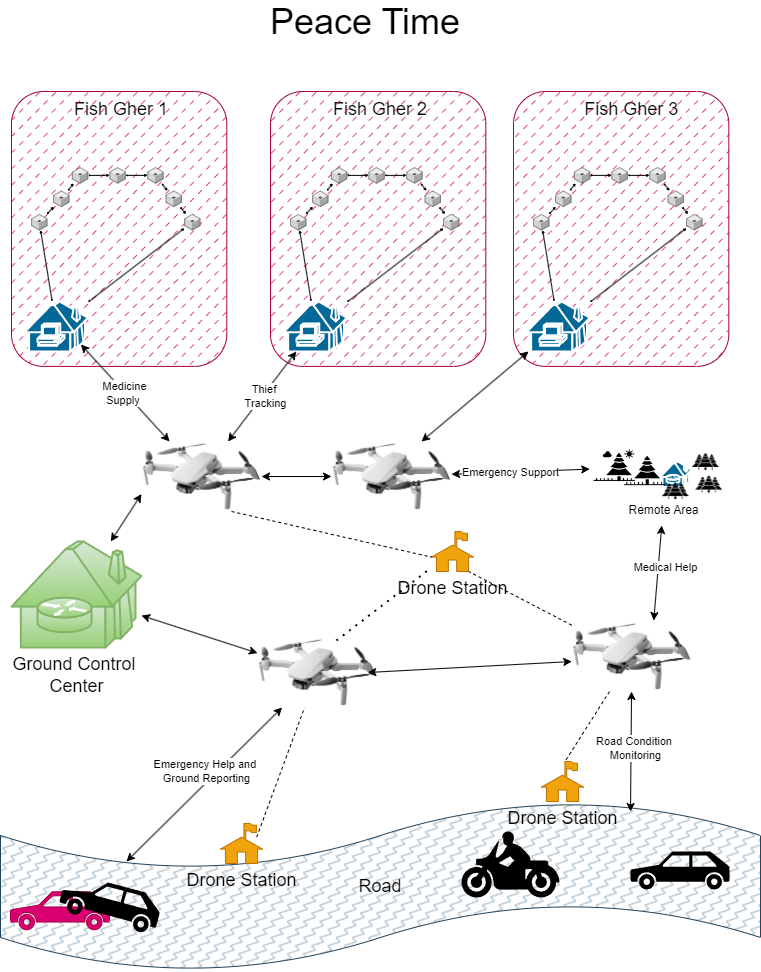
\includegraphics[width=\linewidth]{peace_time.jpg}
    \caption{In the figure, the roles of drones and amphibious unmanned ground vehicles are depicted. During peacetime, the amphibious unmanned ground vehicles will be deployed in Gher farms or aquaculture facilities. Drones will patrol these areas and can also be used for remote emergency medical services and road accident reconnaissance. In the drone station, drones will be stationed, allowing them to recharge their batteries as needed.}
    \label{fig:gher_freshwater}
\end{figure}

\begin{figure}[h]
    \centering
    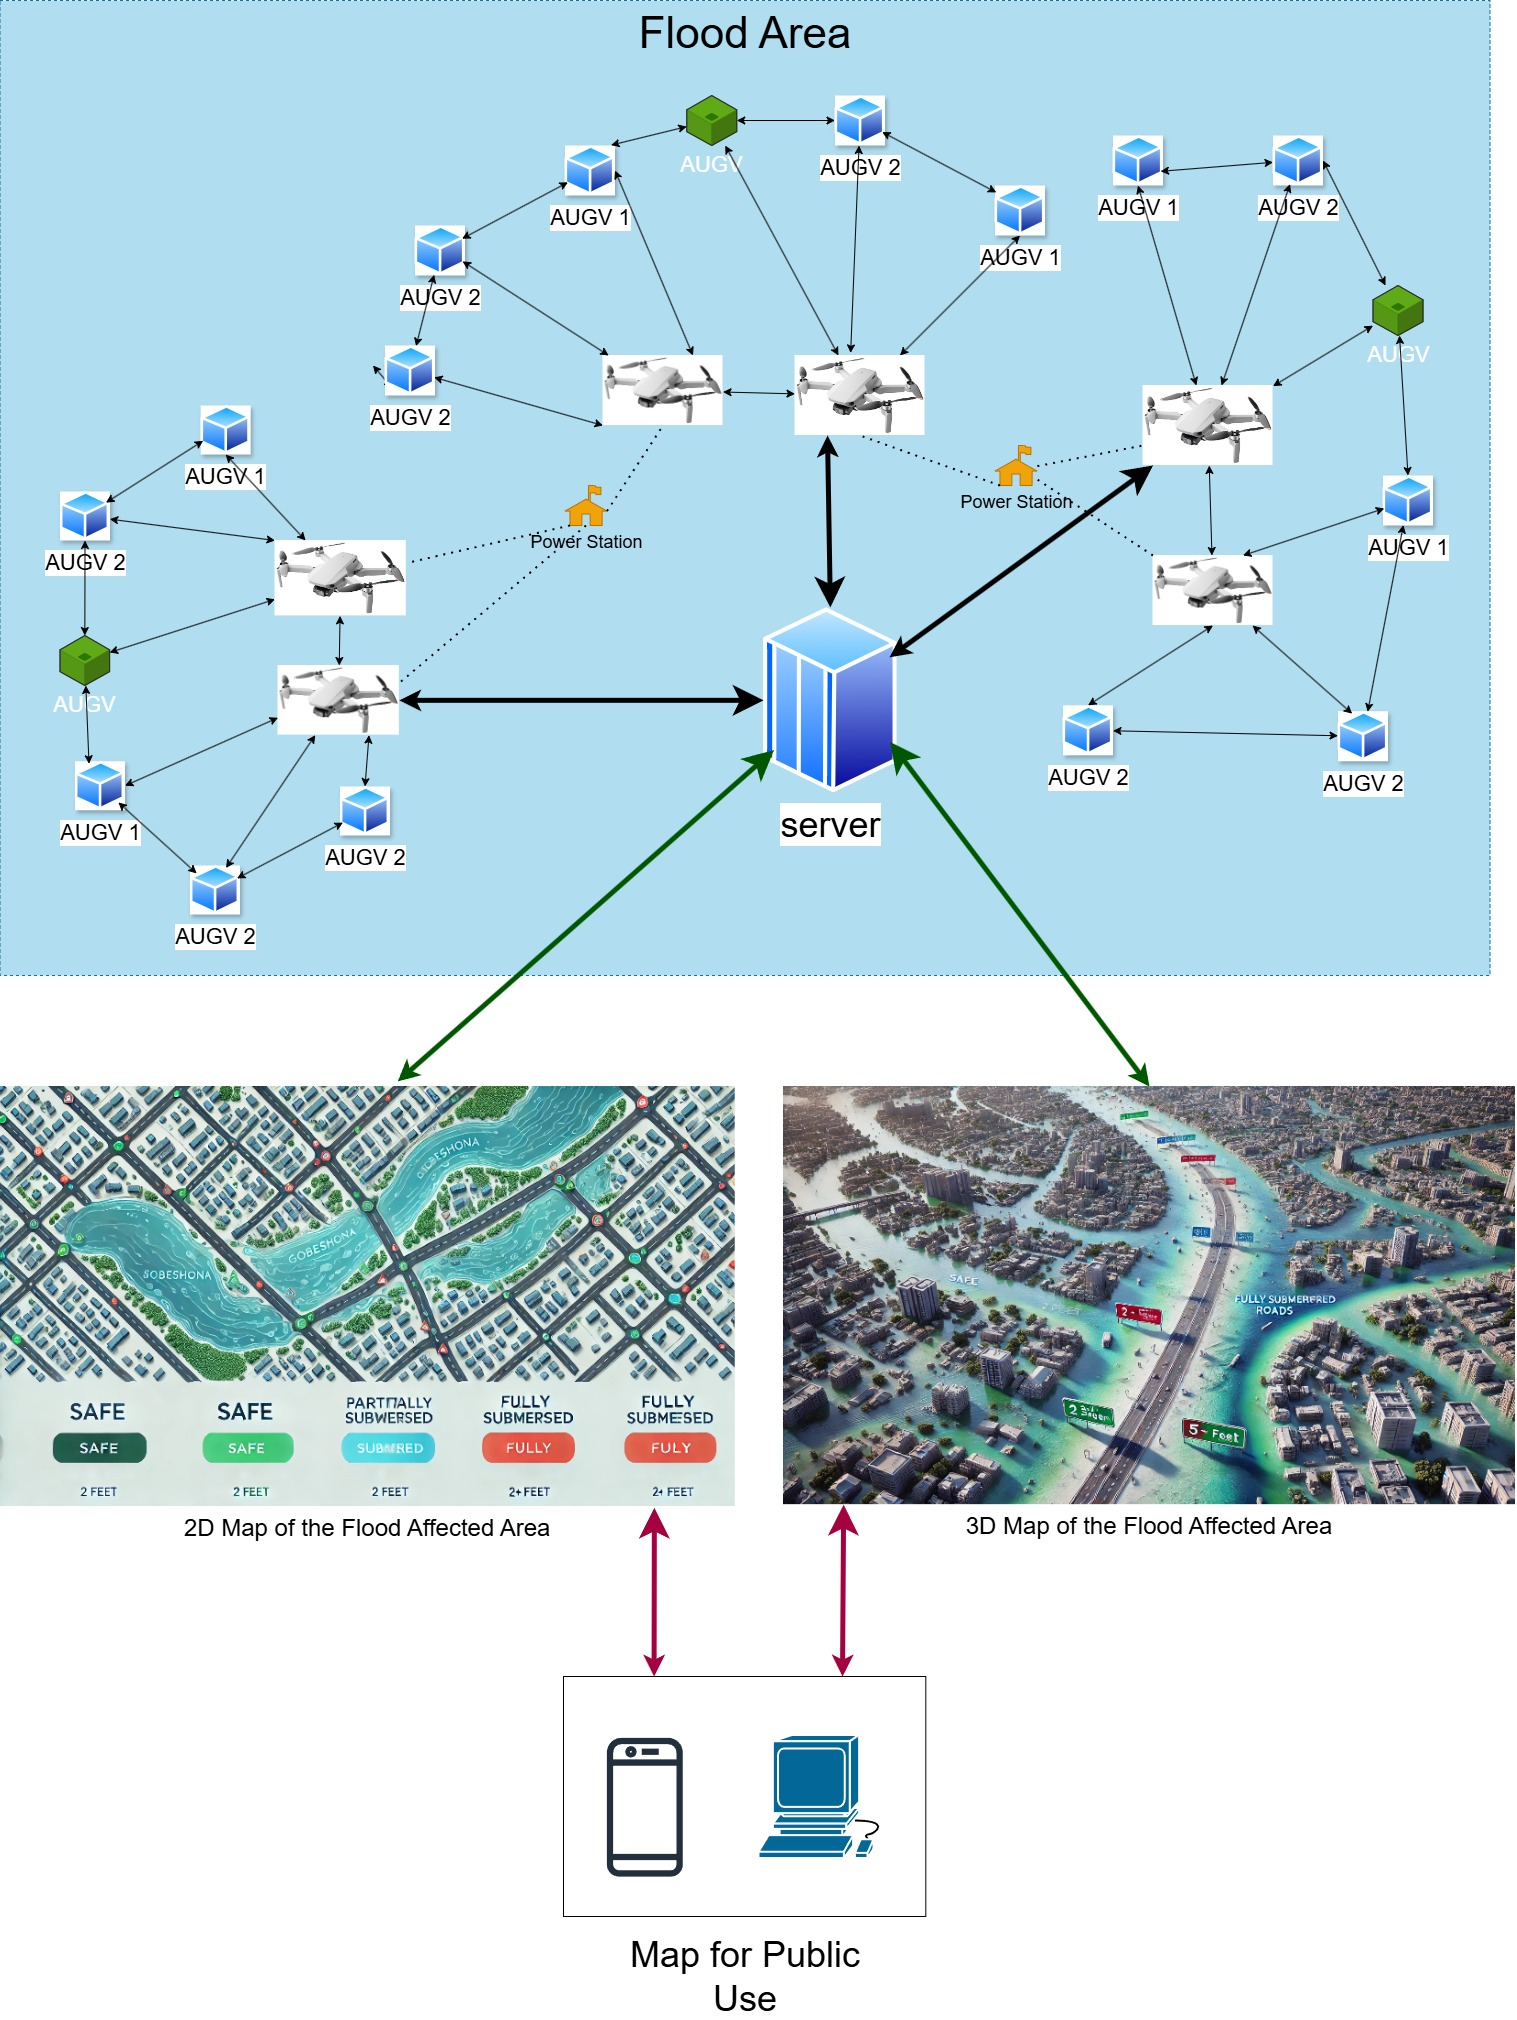
\includegraphics[width=\linewidth]{flood_time.jpg}
    \caption{During flooding, amphibious unmanned ground vehicles (AUGVs) will be deployed for ground reconnaissance in flood-affected areas to detect submerged and dry regions. Drones will provide aerial views. Data from both ground and aerial sources will be combined to generate a comprehensive map. This map will be made publicly available to assist with rescue operations, relief efforts, and for relatives of those in the affected areas.System and the others }
    \label{fig:gher_freshwater}
\end{figure}

	
	
\section{\textbf{Proposed Outcomes}}
The proposed autonomous UAV-UGV system is designed to address critical challenges in both Gher farming and flood management, providing an integrated solution with year-round utility. The anticipated outcomes of implementing this system include:
\begin{enumerate}
	\item \textbf{Enhanced Agricultural Security and Monitoring in Gher Farming}
	The deployment of IoT-based sensors, sonar-based fish monitoring, and AI-driven anomaly detection will offer Gher farmers a robust and automated method to monitor water quality, prevent contamination, and track fish stock health. The system will enable early identification of water contamination and poisoning risks, allowing farmers to respond promptly. The use of autonomous UGVs for continuous 3D mapping will also ensure that any damage to embankments or unwanted objects within the Gher are detected immediately, minimizing economic losses and enhancing overall farm security.
	\item \textbf{Real-Time Flood Mapping and Disaster Management Capabilities}
	During flood events, the UAV-UGV coordination will provide real-time, high-resolution maps of submerged and safe areas, facilitating more effective disaster response. This includes providing accessible, up-to-date maps for emergency teams and farm owners via a web-based interface, detailing navigable routes and high-risk zones. The amphibious UGVs equipped with sonar will allow detailed mapping of submerged terrain, giving relief teams a precise understanding of underwater conditions for safer navigation and improved rescue operations.
	\item \textbf{Dual-Purpose System for Cost Efficiency and Year-Round Utility}
	By offering functionalities for both agricultural monitoring and disaster management, the system maximizes utility and provides a cost-effective solution for Gher farmers and flood-prone communities. The ability of UGVs to transition from farm monitoring to flood response not only ensures their continuous operation but also prevents the degradation associated with seasonally-used equipment. This dual-purpose approach offers a significant return on investment, making advanced technologies accessible and sustainable for small- to medium-scale farms.
	\item \textbf{Extended Operational Range through Autonomous Battery Swapping}
	The system’s autonomous battery-swapping capabilities will allow for extended operation of UGVs and UAVs, even in remote or disaster-affected areas. The implementation of drone-assisted battery transport and autonomous charging stations will reduce downtime and minimize the need for human intervention, ensuring the system remains operational during critical times. This approach will support long-range disaster response and continuous farm monitoring without interruption, bolstering system resilience and reliability.
	\item \textbf{Global Applicability and Scalability}
	With adaptability for various environments and farming systems, the proposed solution is well-positioned for broader implementation in aquaculture and flood-prone areas worldwide. The system can be scaled and configured to accommodate different farming needs and flood management requirements across regions, providing a versatile solution to enhance food security and disaster preparedness on a global scale.
	\item \textbf{Compliance with Future Regulatory Standards}
	Although specific regulations are beyond the research scope, the system’s modular design and integration capabilities align with future airspace and operational guidelines for autonomous drones. This forward-looking approach positions the system to operate ethically and responsibly as regulatory frameworks develop, ensuring long-term viability and smooth integration with public safety protocols.
	
	In summary, the proposed system offers a multi-functional, scalable solution with practical applications in both Gher farming and flood management, addressing critical challenges while remaining adaptable for global needs in aquaculture resilience and disaster response.

	
		

\end{enumerate}
%\section{\textbf{Proposed Outcomes}}



\begin{thebibliography}{99}

\bibitem{ref1} N. Ahmed, J. Brown, and J. Muir, "Freshwater Prawn Farming in Gher Systems in Southwest Bangladesh," \textit{Aquaculture Economics and Management}, vol. 12, no. 3, pp. 207-223, 2008.

\bibitem{ref2} N. Ahmed, M. Troell, E. H. Allison, and J. F. Muir, "Prawn postlarvae fishing in coastal Bangladesh: Challenges for sustainable livelihoods," \textit{Marine Policy}, vol. 34, no. 2, pp. 218-227, 2010.

\bibitem{ref3} M. Haque, "Integrated rice-fish farming systems in Bangladesh," \textit{Aquaculture Journal}, vol. 54, no. 3, pp. 205-215, 2006.

\bibitem{ref4} M. S. Islam and M. A. Wahab, "Shrimp farming in the coastal areas of Bangladesh: Environmentally sustainable development and management practices," \textit{World Aquaculture}, vol. 36, no. 1, pp. 40-47, 2005.

\bibitem{ref5} S. Rahman and B. K. Barmon, "‘Gher’ Farming System of Bangladesh: A Win-Win Strategy for Agricultural Development," in \textit{Agricultural Policies: New Developments}, New York: Nova Science Publishers, Inc., 2011, pp. 143-169.

\bibitem{ref6} University of Stirling, "Gher farming: A unique agricultural system," University of Stirling. [Online]. Available: \url{https://www.stir.ac.uk}. [Accessed: Oct. 20, 2024].

\bibitem{ref7} M. M. Rahman, M. Hasan, and R. Chowdhury, “Climate change and its impact on flooding in Bangladesh,” \textit{Environmental Monitoring and Assessment}, vol. 191, no. 12, p. 729, 2019.

\bibitem{ref8} IPCC, \textit{Climate Change 2021: The Physical Science Basis}. Contribution of Working Group I to the Sixth Assessment Report of the Intergovernmental Panel on Climate Change. Cambridge, U.K.: Cambridge University Press, 2021.

\bibitem{ref9} A. N. Haque and M. S. Ullah, “Flood disaster in Bangladesh: Evaluation of non-structural flood management strategies,” \textit{Natural Hazards}, vol. 102, no. 2, pp. 775–796, 2020.

\bibitem{ref10} S. N. Islam, S. H. Rahman, and Z. Hossain, “Challenges and strategies in flood risk management: A case study of Bangladesh,” \textit{Journal of Flood Risk Management}, vol. 11, no. 3, pp. 1–10, 2018.

\bibitem{ref11} M. R. Khan, M. Roy, and M. Haque, “Role of technology in flood risk management in Bangladesh: Current practices and future prospects,” \textit{Disaster Prevention and Management}, vol. 29, no. 3, pp. 283–297, 2020.

\bibitem{ref12} M. K. Roy, M. I. Hossain, and S. M. Khan, “Autonomous flood monitoring system: Challenges and prospects in Bangladesh,” \textit{IEEE Trans. Intell. Transp. Syst.}, vol. 23, no. 1, pp. 150–162, 2022.

\bibitem{ref13} S. Goddard, P. Shaw, and K. Yim, "Real-time sonar technology in aquaculture: A review of applications and advancements," \textit{Fisheries Science Review}, vol. 62, no. 1, pp. 10-25, 2018.

\bibitem{ref14} P. Butcher and J. Blewett, "Scalable and cost-effective sonar systems for aquaculture security," \textit{Aquaculture Engineering Journal}, vol. 47, no. 3, pp. 101-115, 2020.

\bibitem{ref15} M. A. Hossain and M. I. Chowdhury, "Technological innovations for small-scale aquaculture: A critical review of potential solutions," \textit{Journal of Aquaculture Research and Development}, vol. 10, no. 4, pp. 233-244, 2019.

\bibitem{ref16} M. S. Islam, M. M. Rahman, and R. Ahmed, "IoT-based water quality monitoring systems in Bangladeshi aquaculture: Opportunities and challenges," \textit{International Journal of Environmental Monitoring and Analysis}, vol. 9, no. 2, pp. 45-58, 2021.

\bibitem{ref17} P. Ghosh, R. Shaw, and P. Dhara, "Centralized water quality monitoring in aquaculture: A review of technologies and benefits," \textit{Journal of Aquatic Systems}, vol. 41, no. 3, pp. 234-245, 2018.

\bibitem{ref18} T. Nguyen, D. Pham, and A. Le, "IoT-based water quality monitoring systems in aquaculture: Current trends and future prospects," \textit{Journal of Environmental Monitoring}, vol. 15, no. 2, pp. 156-165, 2020.

\bibitem{ref19} P. Kumar, T. Subramani, and R. Ashok, "Autonomous Surface Vehicles (ASVs) for nutrient distribution and water quality monitoring in aquaculture," \textit{Journal of Robotics in Agriculture}, vol. 33, no. 2, pp. 112-125, 2020.

\bibitem{ref20} S. Nakamura, T. Igarashi, and Y. Kobayashi, "The role of autonomous robotic systems in urban flood management," \textit{Urban Environmental Systems}, vol. 18, no. 1, pp. 35-46, 2021.

\bibitem{ref21} A. Ramirez, J. Sun, and P. Duan, "Robotics in aquaculture: Exploring applications in routine and emergency tasks," \textit{Robotics in Aquaculture}, vol. 32, no. 6, pp. 95-110, 2021.

\bibitem{ref22} L. Wang, D. Cheng, and H. Lin, "Machine learning applications in aquaculture security: Detecting fish movement anomalies for theft prevention," \textit{Journal of Aquaculture Technology}, vol. 51, no. 6, pp. 98-107, 2018.

\bibitem{ref23} L. Mao, Z. Yuan, and H. Chen, "Traditional water level management systems in aquaculture: Challenges and future directions," \textit{Aquaculture Science}, vol. 29, no. 4, pp. 78-89, 2019.

\bibitem{ref24} Q. Zhou, L. Zhang, and F. Huang, "Automation in aquaculture: Opportunities and challenges for operational efficiency," \textit{Aquaculture Engineering Journal}, vol. 57, no. 2, pp. 112-129, 2020.

\bibitem{ref25} S. Sarker and N. Chowdhury, "IoT and AI in Aquaculture: Improving Sustainability and Resilience in Asia-Pacific," \textit{Journal of Agricultural Technology}, vol. 15, no. 2, pp. 120-136, 2022.

\bibitem{ref26} Y. Liu and H. Chen, "Enhancing Aquaculture Efficiency with Automated IoT Solutions," \textit{Aquaculture International}, vol. 28, no. 4, pp. 505-520, 2023.

\bibitem{ref27} C. Abeysinghe et al., "Real-time Monitoring for Small-Scale Aquaculture: Current Trends and Future Directions," \textit{Aquaculture Economics \& Management}, vol. 17, no. 3, pp. 213-231, 2021.

\bibitem{ref28} Q. Zhang and X. Li, "Flood Management Using UAV-UGV Integration for Dynamic Mapping in South American Floodplains," \textit{IEEE Transactions on Geoscience and Remote Sensing}, vol. 58, no. 6, pp. 3418-3435, 2020.

\bibitem{ref29} M. Gomez et al., "Multi-Functional UAV-UGV Systems for Flood Emergency Response," \textit{Journal of Natural Hazards}, vol. 12, no. 8, pp. 415-429, 2019.

\bibitem{ref30} S. Patel and R. Kaur, "Amphibious UGVs in Flood Management: Capabilities and Case Studies," \textit{International Journal of Disaster Risk Reduction}, vol. 55, p. 102446, 2021.

\bibitem{ref31} T. Smith et al., "The Economics of Dual-Purpose Autonomous Systems in Developing Regions," \textit{Resource Management Journal}, vol. 19, no. 3, pp. 389-407, 2023.

\bibitem{ref32} A. Rahman and S. Khan, "Cost-Effective Autonomous Monitoring Solutions for Rural Aquaculture," \textit{Journal of Rural Studies}, vol. 37, no. 2, pp. 150-162, 2020.

\bibitem{ref33} K. Nakamura and M. Sugimoto, "Emergency Medical Drone Applications: An Overview of Current Trends," \textit{Journal of Emergency Medical Services}, vol. 15, no. 3, pp. 214-228, 2022.

\bibitem{ref34} M. Islam and S. Roy, "Drone Delivery for Medical Emergencies in Remote Regions: A Case Study," \textit{Journal of Medical Logistics}, vol. 12, no. 1, pp. 22-34, 2023.

\bibitem{ref35} H. Schmidt and M. Weiskopf, "A Regulatory Review of Drone Operations in Public Safety," \textit{Journal of Airspace Management}, vol. 19, no. 4, pp. 291-308, 2021.

\bibitem{ref36} L. Chen et al., "Centralized Drone Networks for Coordinated Emergency Response: A Framework," \textit{IEEE Transactions on Network and Service Management}, vol. 20, no. 1, pp. 145-158, 2023.


\end{thebibliography}

\end{document}
